% Figure: Multiple Entry Points — Final Common Pathway Funnel
% Shows how different ME/CFS precipitants enter through different
% trigger-capable mechanisms but converge on a single final common pathway.

\begin{figure}[htbp]
\centering
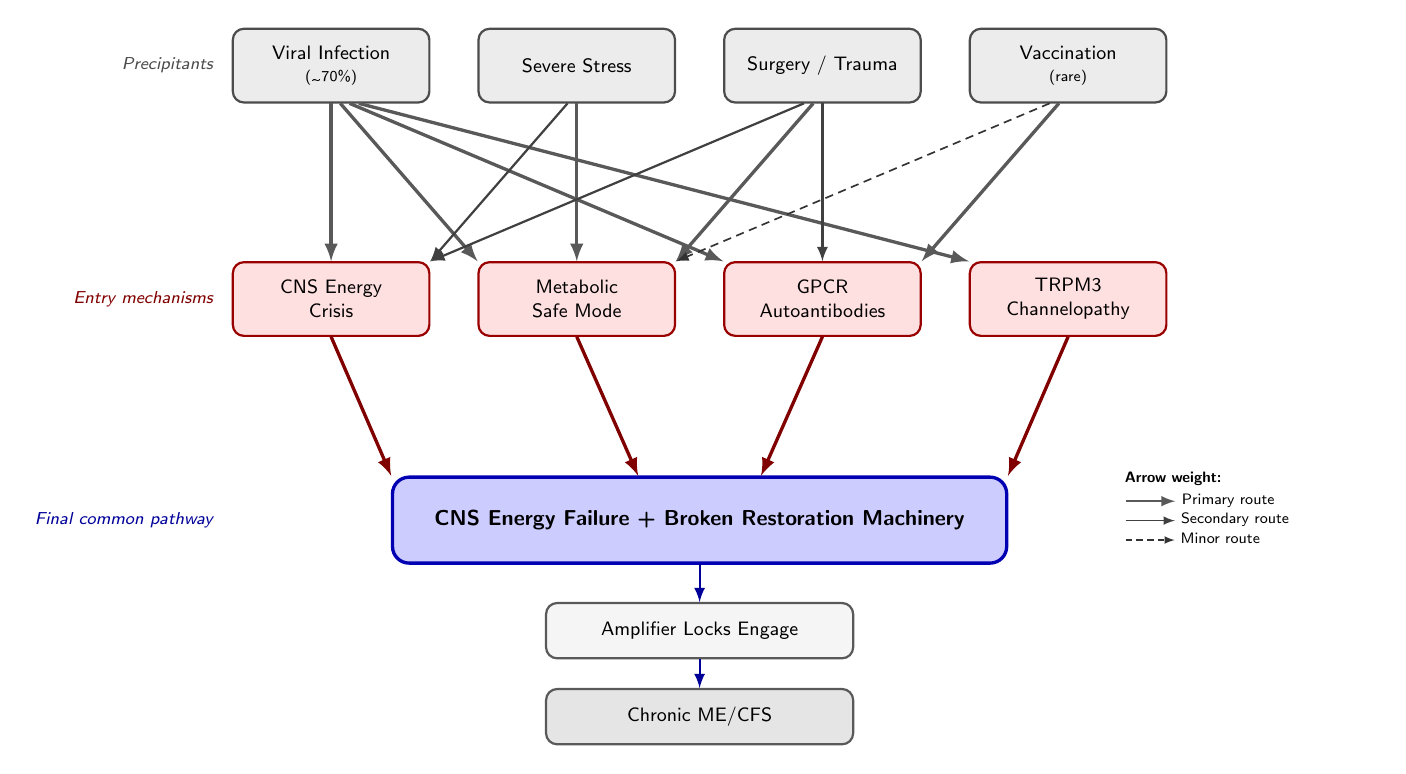
\begin{tikzpicture}[
    scale=0.78, every node/.style={scale=0.78, font=\sffamily},
    % Precipitant boxes (top row, neutral gray)
    precipitant/.style={
        draw=gray!60!black, fill=gray!15, thick,
        rounded corners=4pt,
        minimum width=3.2cm, minimum height=1.2cm,
        align=center, font=\sffamily\small
    },
    % Entry mechanism boxes (middle row, red tones)
    mechanism/.style={
        draw=red!60!black, fill=red!12, thick,
        rounded corners=4pt,
        minimum width=3.2cm, minimum height=1.2cm,
        align=center, font=\sffamily\small
    },
    % Final common pathway (bottom, dark blue)
    pathway/.style={
        draw=blue!70!black, fill=blue!20, very thick,
        rounded corners=6pt,
        minimum width=10cm, minimum height=1.4cm,
        align=center, font=\sffamily\bfseries
    },
    % Outcome box
    outcome/.style={
        draw=gray!70!black, fill=gray!8, thick,
        rounded corners=4pt,
        minimum width=5cm, minimum height=0.9cm,
        align=center, font=\sffamily\small
    },
    % Arrow styles by thickness
    thick arrow/.style={-latex, very thick, gray!70!black},
    medium arrow/.style={-latex, thick, gray!50!black},
    thin arrow/.style={-latex, semithick, gray!40!black, densely dashed},
    % Convergence arrows
    converge/.style={-latex, very thick, red!50!black},
    descend/.style={-latex, thick, blue!60!black},
]

% === TOP ROW: Precipitants ===
\node[precipitant] (viral) at (0, 0)
    {Viral Infection\\[-1pt]{\scriptsize(\texttildelow70\%)}};
\node[precipitant] (stress) at (4, 0)
    {Severe Stress};
\node[precipitant] (surgery) at (8, 0)
    {Surgery / Trauma};
\node[precipitant] (vacc) at (12, 0)
    {Vaccination\\[-1pt]{\scriptsize(rare)}};

% Row label
\node[font=\sffamily\footnotesize\itshape, gray!60!black, anchor=east]
    at (-1.8, 0) {Precipitants};

% === MIDDLE ROW: Entry Mechanisms ===
\node[mechanism] (cns) at (0, -3.8)
    {CNS Energy\\Crisis};
\node[mechanism] (safe) at (4, -3.8)
    {Metabolic\\Safe Mode};
\node[mechanism] (gpcr) at (8, -3.8)
    {GPCR\\Autoantibodies};
\node[mechanism] (trpm) at (12, -3.8)
    {TRPM3\\Channelopathy};

% Row label
\node[font=\sffamily\footnotesize\itshape, red!50!black, anchor=east]
    at (-1.8, -3.8) {Entry mechanisms};

% === ARROWS: Precipitants → Entry Mechanisms ===

% Viral Infection → all 4 (thick)
\draw[thick arrow] (viral.south) -- (cns.north);
\draw[thick arrow] (viral.south) ++(0.15,0) -- (safe.north west);
\draw[thick arrow] (viral.south) ++(0.3,0) -- (gpcr.north west);
\draw[thick arrow] (viral.south) ++(0.45,0) -- (trpm.north west);

% Severe Stress → Safe Mode (thick), CNS (medium)
\draw[thick arrow] (stress.south) -- (safe.north);
\draw[medium arrow] (stress.south) ++(-0.15,0) -- (cns.north east);

% Surgery/Trauma → Safe Mode (thick), CNS (medium), GPCR (medium)
\draw[thick arrow] (surgery.south) ++(-0.15,0) -- (safe.north east);
\draw[medium arrow] (surgery.south) ++(-0.3,0) -- (cns.north east);
\draw[medium arrow] (surgery.south) -- (gpcr.north);

% Vaccination → GPCR (thick), Safe Mode (thin)
\draw[thick arrow] (vacc.south) ++(-0.15,0) -- (gpcr.north east);
\draw[thin arrow] (vacc.south) ++(-0.3,0) -- (safe.north east);

% === BOTTOM: Final Common Pathway ===
\node[pathway] (fcp) at (6, -7.4)
    {CNS Energy Failure + Broken Restoration Machinery};

% Row label
\node[font=\sffamily\footnotesize\itshape, blue!60!black, anchor=east]
    at (-1.8, -7.4) {Final common pathway};

% === CONVERGENCE ARROWS (funnel shape) ===
\draw[converge] (cns.south) -- (fcp.north west);
\draw[converge] (safe.south) -- ([xshift=-1cm]fcp.north);
\draw[converge] (gpcr.south) -- ([xshift=1cm]fcp.north);
\draw[converge] (trpm.south) -- (fcp.north east);

% === BELOW: Chronic outcome ===
\node[outcome] (amplifier) at (6, -9.2)
    {Amplifier Locks Engage};
\node[outcome, fill=gray!20] (chronic) at (6, -10.6)
    {Chronic ME/CFS};

\draw[descend] (fcp.south) -- (amplifier.north);
\draw[descend] (amplifier.south) -- (chronic.north);

% === LEGEND ===
\node[anchor=north west, font=\sffamily\scriptsize, text width=4cm]
    at (12.8, -6.5) {%
    \textbf{Arrow weight:}\\[2pt]
    \tikz[baseline=-0.5ex]{\draw[very thick, gray!70!black, -latex](0,0)--(0.8,0);} Primary route\\[1pt]
    \tikz[baseline=-0.5ex]{\draw[thick, gray!50!black, -latex](0,0)--(0.8,0);} Secondary route\\[1pt]
    \tikz[baseline=-0.5ex]{\draw[semithick, gray!40!black, densely dashed, -latex](0,0)--(0.8,0);} Minor route
    };

\end{tikzpicture}
\caption{Multiple entry points converge on a single final common pathway. Different precipitants preferentially engage different trigger-capable mechanisms, but all converge on CNS energy failure with broken restoration machinery (Section~\ref{sec:entry-points}). Arrow thickness indicates relative likelihood of each entry route.}
\label{fig:entry-points-funnel}
\end{figure}
